\documentclass[conference]{IEEEtran}
\usepackage{cite}
\usepackage{caption}
\usepackage[pdftex]{graphicx}
\usepackage{float}
\usepackage{here}
\usepackage{color}
\usepackage{listings}
\usepackage{algpseudocode}
\usepackage{algorithm}
\usepackage{multicol}
\usepackage{url}
\definecolor{dkgreen}{rgb}{0,0.6,0}
\definecolor{gray}{rgb}{0.5,0.5,0.5}
\definecolor{mauve}{rgb}{0.58,0,0.82}
\topmargin 0mm
\oddsidemargin 5mm
\evensidemargin 5mm
\textwidth 150mm
\textheight 662.801 pt
\lstset{frame=tb,
  language=Java,
  aboveskip=3mm,
  belowskip=3mm,
  showstringspaces=false,
  columns=flexible,
  basicstyle={\small\ttfamily},
  numbers=none,
  numberstyle=\tiny\color{gray},
  keywordstyle=\color{blue},
  commentstyle=\color{dkgreen},
  stringstyle=\color{mauve},
  breaklines=true,
  breakatwhitespace=true
  tabsize=3
}
\begin{document}
\title{Android pedometer application capable of saving data on the Cloud
\begin{figure}[H]
\centering
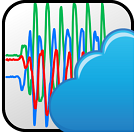
\includegraphics[width=2cm]{Title.jpg}
\end{figure}
}

\author{
\IEEEauthorblockN{MohammadHossein AskariHemmat\\ University of McGill\\ Course Instructor: Dr. Z. Zilic
 }

}
\maketitle

\section{Project Description :}
This document is submitted for the third assignment of ECSE 649 course.  In this assignment we were asked to design an Android Application that is capable of storing the coming data from the mobile sensors into Cloud. We were asked to use BOX~\cite{BoxAppRef}, which is file sharing and cloud content management service, for this purpose. The energy efficiency of the design had to be taken into account. In my case I used the raw data from Linear Accelerometer to design a pedometer~\cite{PedometerRef} application. This way the amount of data that will be stored in the cloud would be decreased. The Pedometer design will be explained in details later in this document.\\
My application includes four major blocks as follows:\\
\begin{itemize}
  \item A Service, which runs in background, that deals with collecting the data from the accelerometer.
  \item A Pedometer that uses the raw data from the service and decides whether the coming data matches with the walking pattern or not.
  \item A Handler that deals with storing the data into the cloud
  \item A Main activity that wraps all the above blocks
\end{itemize}
The rest of this document is going to explain all the above blocks in details. In Figure\ref{ApplicationModules} the overall application layout is illustrated.
\begin{figure}[H]
\centering
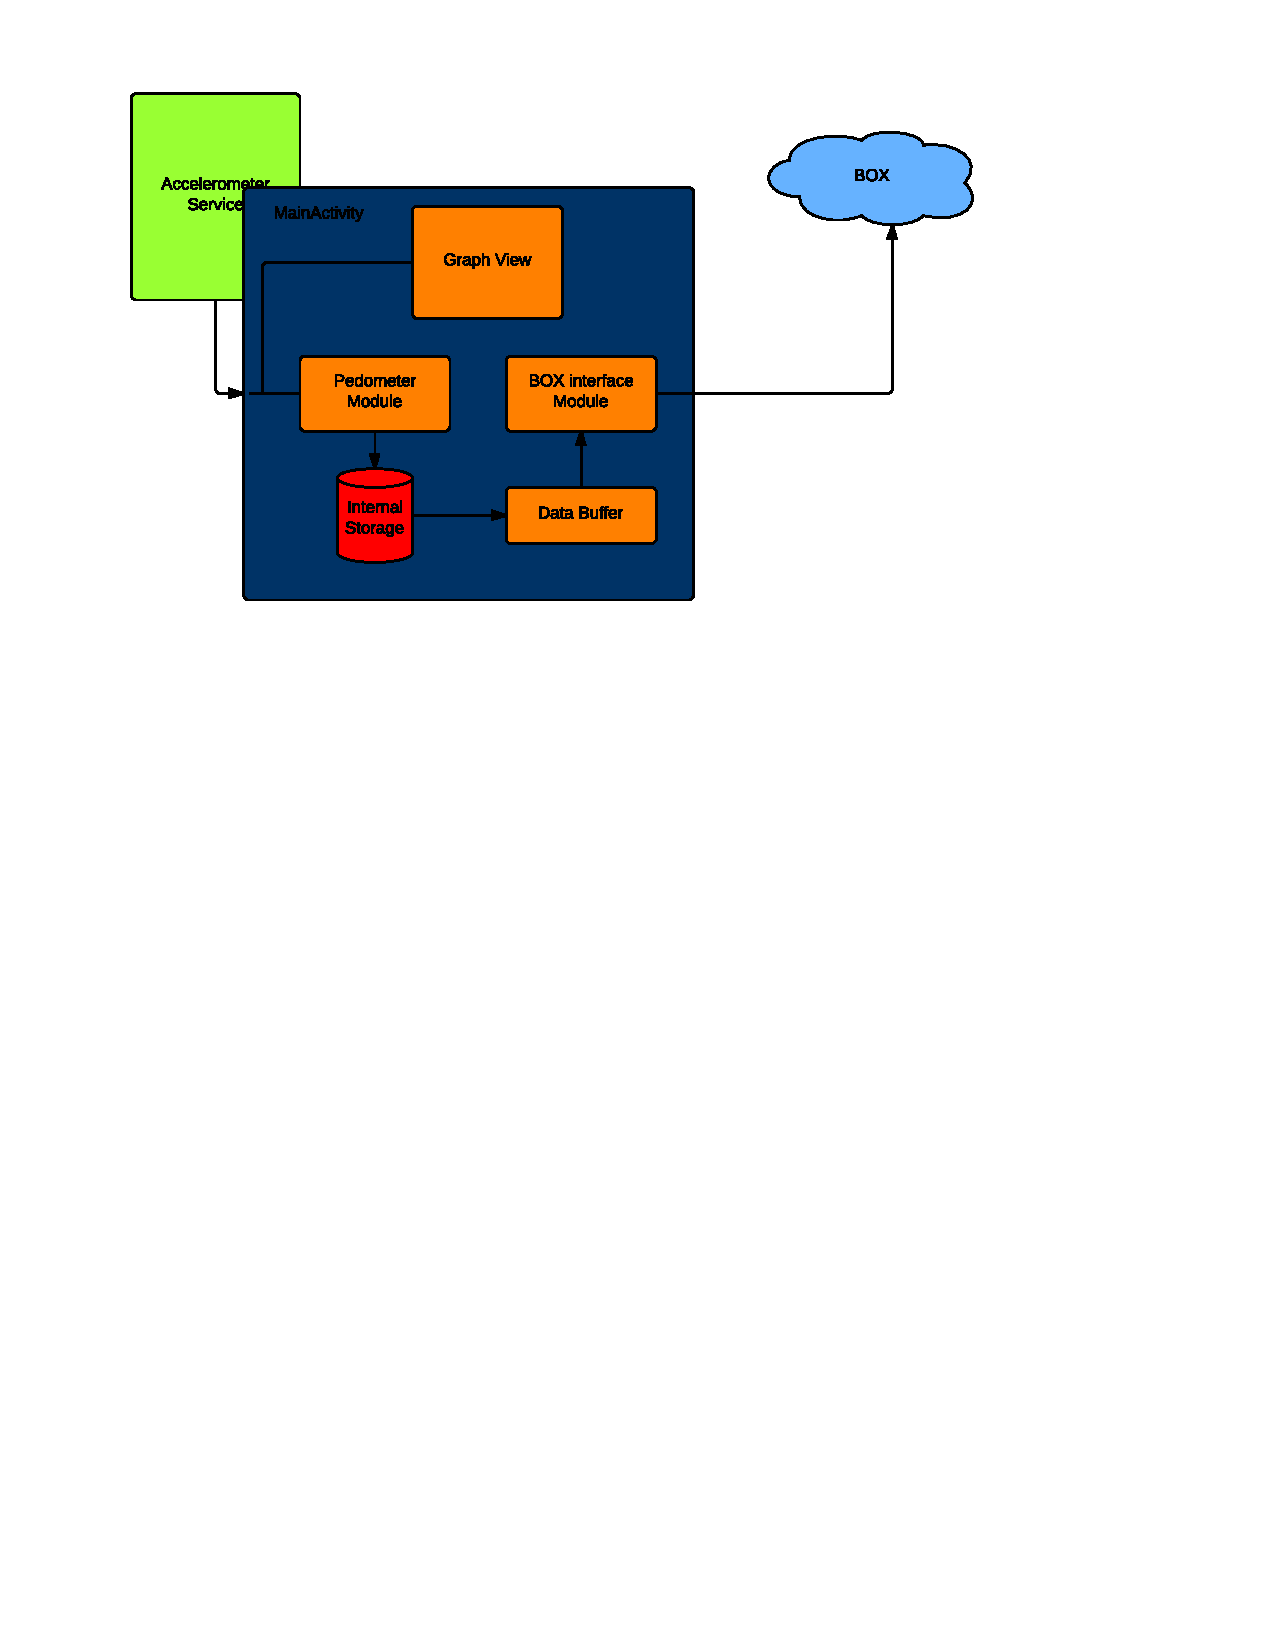
\includegraphics[width=9cm]{OverallApplicatio.pdf}
\caption{\scriptsize  Application Modules}
\label{ApplicationModules}
\end{figure}

\section{Collecting data from Accelerometer}
One of the best ways to collect data from a hardware resource is to use a service in background. The service should be capable of collecting the data from the hardware and then send it to the activities that are binded to the service. Also, the service should be capable of registering to and unregistering from the Hardware when ever it is needed. For instance assume that the battery level is low and the user don't need to collect the data from accelerometer anymore. At the same time he/she needs to use some of the application features regardless of the accelerometer data. It will be very convenient to let user to disable or enable the accelerometer at any time. In my design, user can do the latter by going to the application settings and from there disable or enable the hardware. The settings is illustrated in Figure\ref{DisEnAccel}. In android simply you can enable or disable a hardware resource by unregistering the from the listener list.
\\It is important to know that Android will not let you to power down the Acceleromter sensor. The reason is that there are other applications that are using the accelerometer data and by turning down the accelerometer, the functionality of other applications will be affected. \\
\begin{figure}[H]
\centering
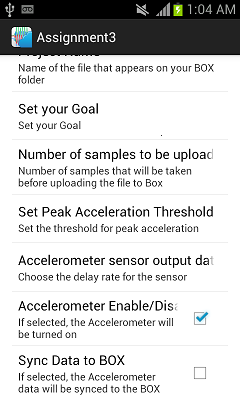
\includegraphics[width=4cm]{DisEnAccel.jpg}
\caption{\scriptsize  Disable/Enable Accelerometer sensor}
\label{DisEnAccel}
\end{figure}
The other way that can do the same thing is to unbind the main activity from the accelerometer service. But the difference is that the serivce will keep collecting data but it would not send them to the activity. Clearly, this is not an efficient way in terms of power consumption.\\
The  other way to save power is by reducing the output data rate of the module. I have also added this feature to my application so that the user could have a number of choice in case that he/she is running out of battery. Android provides four output data rate as illustrated in Figure\ref{DisEnAccel}
\begin{figure}
\centering
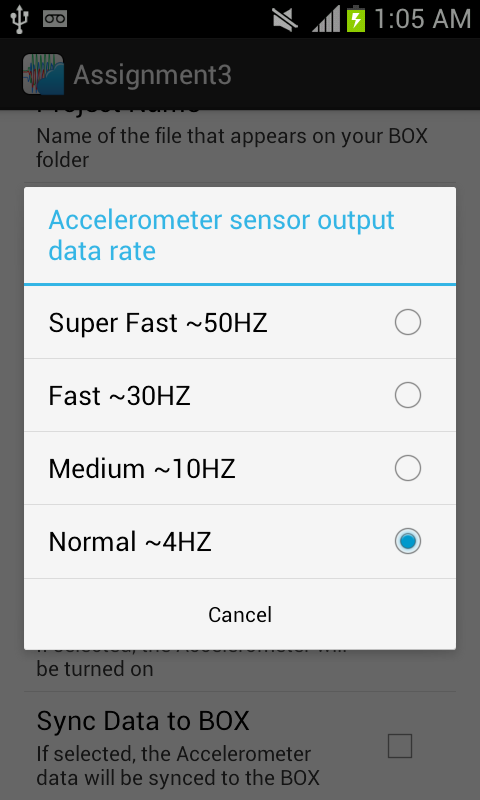
\includegraphics[width=4cm]{DataRate.jpg}
\caption{\scriptsize  Acceleromter output data rate}
\label{DisEnAccel}
\end{figure}
Overall, in order to save power, one of my strategies was to provide the user with some hardware control so his/her decisions can affect the overall power consumption. By default, the acceleromter is turned off and the slowest data rate is selected.

\section{Pedometer Module}
A pedometer is a device, usually portable and electronic or electromechanical, that counts each step a person takes by detecting the motion of the person's hips~\cite{PedometerRef}. Currently, using 3-Axis accelerometer is a common way to count the number of steps. One of the biggest problem using accelerometer data in a pedometer is filtering the effect of gravity. Usually an extra hardware/software high pass filter is used to filter out the DC component and based on this result. The other way to solve this problem is to use a linear accelerometer instead. The linear accelerometer can be implemented in hardware or in software. The difference with a common accelerometer is that you do not need any extra piece of Hardware or Software to obtain the accelereation excluding the force of gravity. As a hardware Linear Acceleromter LIS3LV02DL~\cite{STACCEL} from ST is good example. The Circuit Diagram of this module is illustrated in Figure\ref{STACCEL}
\begin{figure}[H]
\centering
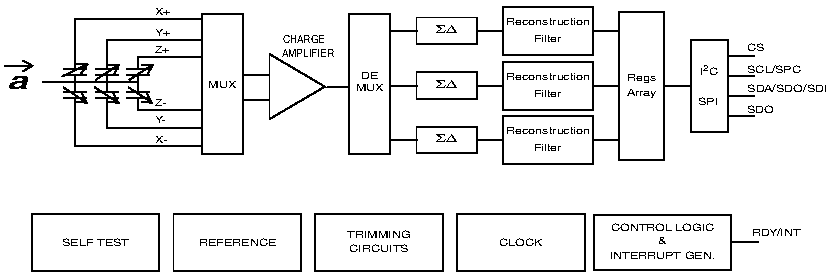
\includegraphics[width=11cm]{STLinearAccel.pdf}
\caption{\scriptsize  LIS3LV02DL Circuit Diagram}
\label{STACCEL}
\end{figure}
It can be seen from the Circuit Diagram  that a hardware $\Sigma\Delta$ and Reconstruction is used to filter the effect of gravity. As an example of software Linear accelerometer, Google provided this sensor in Android and it can be accessed using \textcolor{blue}{\emph{TYPE\_LINEAR\_ACCELERATION}}. In my application, I used Google Linear Acceleration sensor type in my application. A Google Tech Talks of Linear acceleromter can be found in~\cite{LinearAccel}.\\
The raw data from the Linear acceleromter still cannot be used in a pedometer application. In my application I used an FIR filter to smooth out the raw data from the Linear acceleration sensor and then I feed this data into the pedometer module.  To find out how to count a change in acceleromter data as a step or not, We need to understand the pattern of walking. In ~\cite{PedPatternRec} this pattern has been explained. Based on the model that is presented in latter paper, I came up with a fairly stable algorithm. The algorithm is illustrated in Figure~\ref{PedAlg}.\\
\begin{figure}[H]
\centering
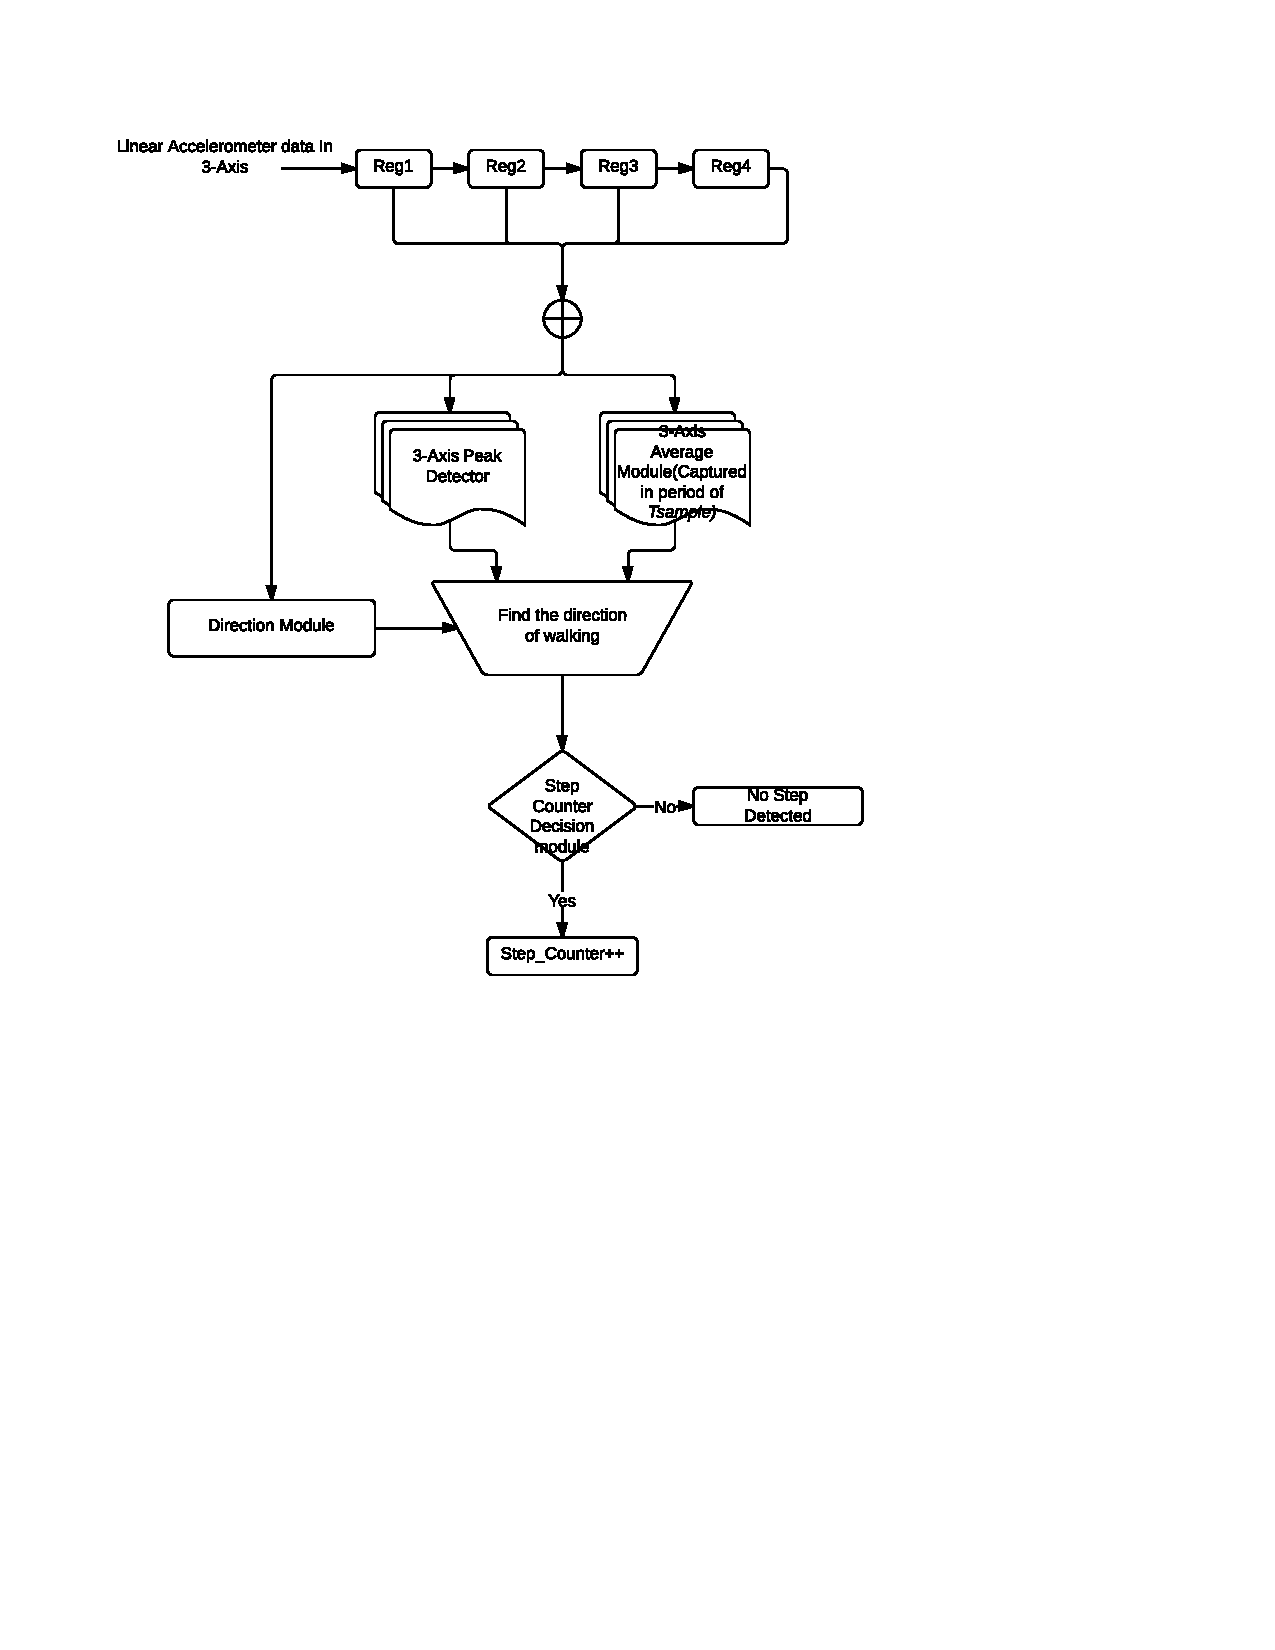
\includegraphics[width=8cm]{PedometerAlg.pdf}
\caption{\scriptsize  Pedometer Algorithm}
\label{PedAlg}
\end{figure}

First the acceleromter data is passed threw an FIR filter. Then it passes threw 3 modules as follow:
\begin{itemize}
  \item Peak Detector Module
  \item Averaging Module
  \item Direction Module
\end{itemize}

All the above modules are working on the 3-Axis filtered acceleration data. Since the rate of data is not constant, the averaging is done based on the data rate that the user has been selected. Considering that the average delay between each step is around 1 second (based on my experience) I used the following formula to find the number of samples that has to be averaged each time:
\begin{equation}\label{eq1}
StepSampleRate = StepInterval*DataRate;
\end{equation}
I set the StepInterval to 1 second and DataRate will be updated each time that the user modifies his/her accelerometer output data rate.
The averaging module output and the peak detector output modules are fed to a decision module that decides in which direction change has been occurred. This decision is based on the output of the Direction Module. After finding out the direction of change, the corresponding data is fed into the Step Counter Decision Module. In this module, based on the Peak acceleration threshold, it is decided whether the input data should be count as a step or not. A sample data output from all the major blocks is illustrated in Figure\ref{DataOut}. This figure was captured from the \emph{DATAGRAPH} in the application
\begin{figure}
\centering
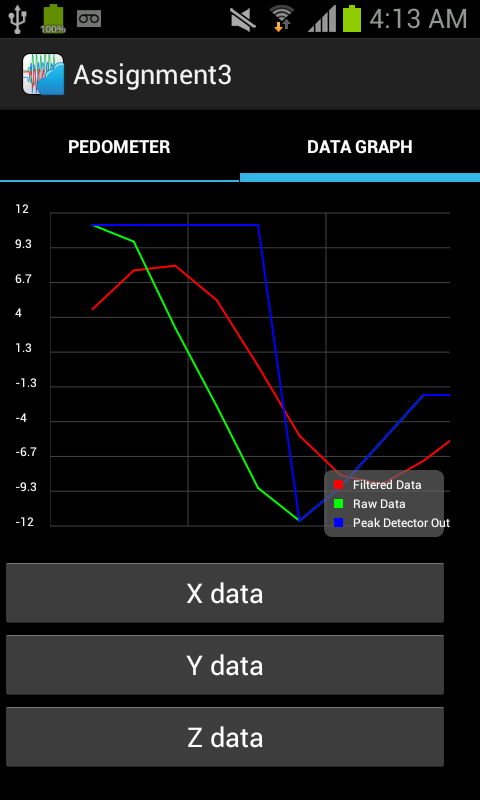
\includegraphics[width=5.5cm]{DATAGRAPH.jpg}
\caption{\scriptsize  Output data from the Pedometer algorithm blocks}
\label{DataOut}
\end{figure}
Based on my experience, the algorithm works best by setting the Data rate to 30HZ and setting the Peak acceleration data to around 1.2. These parameter can be modified in the application's settings. Also it is available for the user to set a Goal for the number of steps. The Pedometer graphical user interface is illustrated in Figure\ref{Pedgui}.
\begin{figure}
\centering
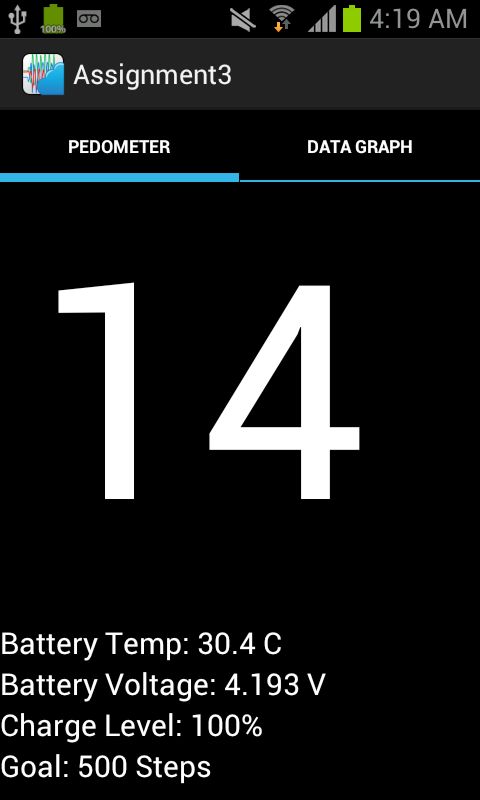
\includegraphics[width=5.5cm]{PedometerGUI.png}
\caption{\scriptsize  Pedometer GUI}
\label{Pedgui}
\end{figure}
\section{BOX Interface Module}
In order to process/store the data in it is very practical to use a cloud service. In this assignment we used BOX as a cloud storage service. BOX platform supports many other platfroms such as: Android, iOS, Windows and etc. Since we are creating an Android application, we need to download and install BOX Android SDk on the ADT. Here is a link to the SDK in Github:\\\url{https://github.com/box/box\-android\-sdk\-v2}. All the infromation for setting the BOX Android SDk is covered.\\
 In order to interact with BOX platform, first we need to create an account in BOX. BOX uses OAuth 2.0 to authenticate and authorize the access of the users to the their account. Applications needs to be aware of three parameters in order to use OAuth:
\begin{itemize}[h]
  \item Client ID
  \item Client Secret
  \item Redirect Url
\end{itemize}
Before accessing to BOX using OAuth, its needed to create a Box Application. The later parameters are set in this stage. We need to them in the OAuth parameters section. The Client ID and Client secret ID are generated automatically. But the Redirect url has to set manually. The redirect URI is the URL within your application that will receive the OAuth2 credentials~\cite{BoxAppRef}. For most application \textcolor{blue}{http://localhost} can be set as the Redirect Url parameter. After creating the application in the BOX account, now we need to copy and store these information into the BOX client parameters in our Android application.\\
To access our Application in BOX, first we need to authenticate our access. This is simply done by starting an OAuthActivity in Android and then call the suitable method based on the response from BOX. Here is Pseudo code:
\begin{lstlisting}

public void StartAuth(){
Intent intent = OAuthActivity.createOAuthActivityIntent(CLIENT ID,SECRET_ID,url);
this.startActivityForResult(intent,AUTH_REQUEST); 				
}

// After responding BOX to our request:
private void onAuthenticated(int resultCode, Intent data) {
      if (Activity.RESULT_OK != resultCode) {
          authentication = false;
	         }
	         else {
	             BoxAndroidClient client = new BoxAndroidClient(BoxClient.CLIENT_ID, BoxClient.CLIENT_SECRET, null, null);
	             client.authenticate(oauth);
	             if (client == null) {
	                 authentication = false;
	             }
	             else {
	             	((BoxClient)getApplication()).setClient(client);
	                 authentication = true;
	             }
	         }
	     }
\end{lstlisting}

If the authentication was successful, we will able to perform Upload, Download and other methods that are provided by the BOX platform. In my application, authentication will be saved after the first successful access. If the user exits the application, the authentication will be deleted. If he/she preferred to run the application in the background, no authentication will be asked after his/her return. Also it is available to use the application without Syncing the data to the BOX. To do so, user need to Uncheck the SynC Data to BOX option in the settings. In order to save power, user can set the\emph{Number of samples to be uploaded } parameter in the settings menu. This parameter determines how frequent data should be uploaded into the BOX. The minimum value for this parameter is 500 samples which will give only 1 second before each data uploading. By setting this parameter to 500, the power consumption will increase very fast. The default value is 2000. Also to save power, only the number of steps are sent to be stored.
 Figure~\ref{NoSamples} shows the setting of this option:
\begin{figure}
\centering
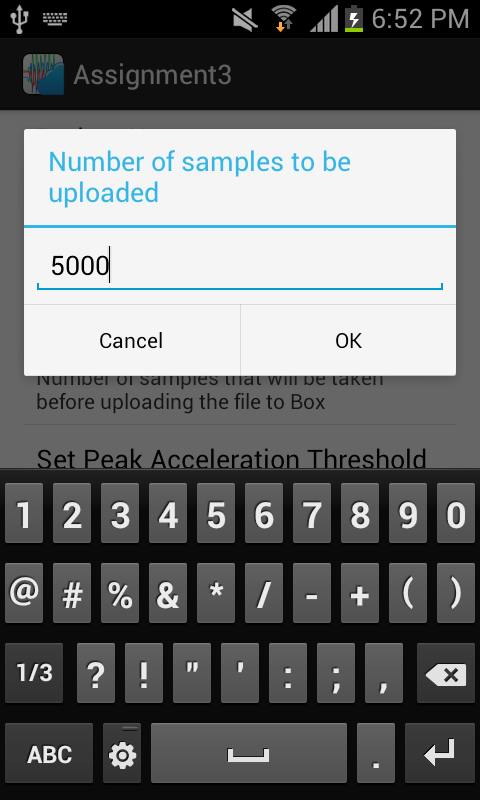
\includegraphics[width=5.5cm]{NumbefOfSamples.png}
\caption{\scriptsize setting the Number of samples to be uploaded }
\label{NoSamples}
\end{figure}
The name of file that will be saved into the BOX can also be defined.
To avoid losing data while Syncing data to BOX, I Used a File buffer. So the pedometer save its data to a buffer and the BOX interface reads it only if its available.
\newpage
\section{Main Activity}
All of the above modules Plus the DataGraph modules are controlled by the main activity. Main activity is responsible to save/delet the files from the external storage device. It is also responsible to save the authentication and ask for re-authentication if its needed.
\section{Conclusion}
in this assignment we learned how to use a cloud service to save our data from our android application. We were asked to try to design the most efficient application in terms of power consumption. My application run for 11 hours non-stop in the most power consuming settings which is uploading data every 1s and set the Linear acceleromter data rate to 50HZ. 

%=============================================================================================
\begin{thebibliography}{1}
%=============================================================================================
%1
\bibitem{BoxAppRef}
https://app.box.com/
%=============================================================================================
%2
\bibitem{PedometerRef}
http://en.wikipedia.org/wiki/Pedometer
%=============================================================================================
%3
\bibitem{STACCEL}
http://www.st.com/web/catalog/sense\_power/FM89/SC444/PF127514?referrer=70032480
%=============================================================================================
%4
\bibitem{LinearAccel}
https://www.youtube.com/watch?v=C7JQ7Rpwn2k\&feature=player\_detailpage\#t=1349
%=============================================================================================
%5
\bibitem{PedPatternRec}
N.Zhao, "Full-Featured Pedometer Design Realized with 3-Axis Digital Accelerometer",Analog Dialogue 44-06, June (2010)


\end{thebibliography}

\end{document}
